% \pagebreak[4]
% \hspace*{1cm}
% \pagebreak[4]
% \hspace*{1cm}
% \pagebreak[4]
\chapter{Literature Review}
%\ifpdf
%    \graphicspath{{Literature/LiteratureFigs/PNG/}{Literature/LiteratureFigs/PDF/}{Literature/LiteratureFigs/}}
%\else
%    \graphicspath{{Literature/LiteratureFigs/EPS/}{Literature/LiteratureFigs/}}
%\fi




The very famous quote of, ``To err is human, but to really foul things up you need a computer", is quite relevant to the software programmers. Programmers being humans are prone to errors. Errors are not tolerated, particularly in software because a single error may cause a large upset in the system. According to the National Institute of Standard and Technology 2002, software errors cost an estimated \$59.5 billion loss to US economy annually. The destruction of the Mariner 1 rocket (1962) costing \$18.5 million was due to a small error in formula coded incorrectly by programmer. The Hartford Coliseum Collapse (1978) costing \$70 million, Wall Street crash (1987) costing \$500 billion, failing of long division by Pentium (1993) costing \$475 million, Ariane 5 Rocket disaster costing \$500 million are a few examples of losses caused by minor errors in the software. To achieve high quality, the software has to satisfy rigorous stages of testing. The more critical and complex the software, the higher the requirements for software testing and the larger the extent of damage caused as a result of an error in the software.

\section{Software Testing}
In the IEEE standard glossary of software engineering terminology~\cite{american1984}, testing is defined as ``the process of exercising or evaluating a system or system component by manual or automated means to verify that it satisfies specified requirements and actual results. A successful test is one that finds a fault~\cite{Myers2004}, where fault is defined as, the error made by people during software development~\cite{american1984}.

Being an integral part of Software Development Life Cycle (SDLC), the testing process starts from requirement phase and continues throughout the life of the software. In traditional testing when tester finds a fault in the given SUT, the software is returned to the developers for rectification and is consequently given back to the tester for retesting. It is important to note that, ``program testing can be used to show the presence of bugs, but never to show the absence of bugs"~\cite{Dijkstra1972}. In other words, a SUT that passes all the tests without giving a single error is not guaranteed to contain no error. However, the testing process increases the reliability and confidence of users in the tested product.

\begin{table}[ht]
%\scriptsize
\caption{Parts of Software Testing~\cite{adrion1982validation},~\cite{chilenski1994applicability},~\cite{gaudel2010software},~\cite{richardson1992specification},~\cite{tracey1998automated}} % title of Table
\smallskip
\centering % used for centering table
\begin{tabular}{| l | l | l | l | } % centered columns (4 columns)
\hline

Levels 		&Purpose		 						& Perspective		& Execution 	\\
\hline
1. Unit		&1. Functionality						& 1. White Box		& 1. Static 	\\
2. Integration	&2. Structural							& 2. Black Box		& 2. Dynamic	\\
3. System		&3. Robustness						& 3. Grey Box		&			\\
			&4. Stress								&				&			\\
			&5. Compatibility						&				&			\\
			&6. Performance						&				&			\\



\hline %inserts single line
\end{tabular}
\bigskip
\label{table:addvalues} % is used to refer this table in the text
\end{table}


\subsection{Software Testing Levels}
The three main levels of software testing defined in the literature include unit testing, integration testing and system testing~\cite{chilenski1994applicability}. Unit testing involves evaluation of piece-by-piece code and each piece is considered as independent unit. Units are combined together to form components. Integration testing ensures that the integration of units in a component is working properly. System testing is called out to make sure that the system formed by combination of components performs correctly to give the desired output.

\subsection{Software Testing Purpose}
The primary purpose of software testing is identification of faults in the given SUT for necessary correction in order to achieve high quality. Maximum number of faults can be identified if software is tested exhaustively. In exhausting testing SUT is checked against all possible combinations of input data, and the results obtained are compared with the expected results for assessment. Exhaustive testing is not always possible in most scenarios because of limited resources and infinite number of input values that software can take. Therefore, the purpose of testing is generally directed to achieve confidence in the system involved from a specific point of view. For example, functionality testing is performed to check functional aspect for working correctly. Structural testing analyses the code structure for generating test cases in order to evaluate paths of execution and identification of unreachable or dead code. In robustness testing the software behaviour is observed in the case when software receives input outside the expected input range. Stress and performance testing aims at testing the response of software under high load and its ability to process different nature of tasks~\cite{cohen2005robustness}. Finally, compatibility testing is performed to see the interaction of software with underlying operating system.
 %As proper planning is the key to success for many projects this is often also true with software testing. A software test plan is a well defined document that defines the goal, scope, method, resources and time schedule of the testing.
%A software testing technique in which a software is tested with all possible combination of inputs. This technique can prove conclusively that the software meet its specification however exhaustive testing is seldom feasible because of the large input domain or too many paths in a software code. 

\subsection{Software Testing Perspective}
Testing activities can be split up into white-box and black-box testing on the basis of perspective taken. 

\subsubsection{White-box testing}
In white-box or structural testing, the testers must do need to know about the complete structure of the software and can do necessary modification, if so required. Test cases are derived from the code structure and test passes only if the results are correct and the expected code is followed during test execution~\cite{ostrand2002white}. Some of the most common White-box testing techniques are briefly defined:

\paragraph{Data Flow Analysis}
Data Flow Analysis is a testing technique that focuses on the input values by observing the behaviour of respective variables during the execution of the SUT~\cite{clarke1989formal}. In this technique a control flow graph (CFG), graphical representation of all possible states of program, of a SUT is drawn to determine the paths that might be traversed by a program during its execution. Test cases are generated and executed to verify its conformance with CFG on the basis of data. 

Normally, program execution implies input of data, operations on it according to the defined algorithm, and output of results. This process can be viewed as a flow of data from input to output in which data may transform into several intermediate results before reaching its final state. In the process several errors can occur e.g. references may be made to variables that don’t exist, values may be assigned to undeclared variables or the value of variables may be changed in an unexpected and undesired manner. It is the ordered use of data implicit in this process that is the central object of the technique to ensure that none of the aforementioned errors occur~\cite{fosdick1976data}.

\paragraph{Control flow analysis}
Control flow Analysis is a testing technique which takes into consideration the control structure of a given SUT. Control structure is the order in which the individual statements, instructions or function calls are executed. In this technique a control flow graph (CFG), similar to the one required in data flow analysis, is drawn to determine the paths that might be traversed by a program during its execution. Test cases are generated and executed to verify its conformance with CFG on the basis of control. For example to follow a specific path (also known as branch) between two or more choices at specific state. Efforts are made to ensure that the set of selected test cases execute all the possible control choices at least once. The effectiveness of the testing technique depends on controls measurement. Two of the most common measurement criteria defined by Vilkomir et al. are Decision/Branch coverage and Condition coverage \cite{vilkomir2003tolerance}. 

\paragraph{Code-based fault injection testing}
A technique in which additional code is added to the code of the SUT at one or more locations to analyse its behaviour in response to the anomaly \cite{voas1997software}. The process of code addition is called instrumentation which is usually performed before compilation and execution of software. The added code can be use for multiple reasons i.e. injection of fault to find the error handling behaviour of software, to determine the effectiveness of test procedure to check whether it discover the injected faults or to measure the code coverage achieved by the testing process.    

\subsubsection{Black-box testing}
In black-box or functional testing, the testers do not need to know about internal code structure of the SUT. Test cases are derived from the specifications and test passes if the result is according to expected output. Internal code structure of the SUT is not taken into any consideration~\cite{beizer1995black}. Some of the most common black-box testing techniques are briefly defined:

\paragraph{Use-case based testing}
A verification and validation technique that utilizes use-cases of the system to generate test cases. Use-case define functional requirements at a particular situation or condition of the system from actor's (user or external system) perspective. It consists of a sequence of actions to represent a particular behaviour of the system. A use case format include a brief description of the event, flow of events, preconditions, postconditions, extension points, context diagram and activity diagram. 
All the details required for test case is included in the use case therefore use case can be easily transformed into test case. 

% steps taken from presentation of Raional User Conference 2003. Check it for viva.

The main benefits of use case testing is cheap generation of test cases, avoidance of test duplication, improved test coverage, easier regression testing and early identification of missing requirements.  

\paragraph{Partition testing}
A testing technique in which the input domain of a given SUT is divided into sub-domain according to some rule and then tests are conducted in each sub-domain. The division in to sub-domain can be according to the requirements or specifications, structure of the code or according to the process by which the software was developed \cite{{hamlet1990}. 

While the performance of partition testing is directly dependant on the quality of sub-domain \cite{weyuker1991analyzing}, it is often however difficult to divide the domain into equal partitions. Therefore, another version of partition testing called Proportional sampling strategy: guidelines for software testing practitioners \cite{Chan1996} is devised, in which the number of test cases selected from each partition is directly proportional to the size of the partition. Experiments performed by Ntafos \cite{ntafos1998random} confirm the better performance of proportional partition testing over partition testing.


\paragraph{Boundary value analysis}
Boundary Value Analysis (BVA) is a testing technique which is based on the rationale that errors tends to occur near the extremities of the input variables. Therefore in BVA the data set consists of values which are selected from the borders. According to IEEE standards \cite{radatz1990ieee}, boundary value is a value that corresponds to minimum or maximum input, internal or external value specified for a component or system. 

The BVA technique is also used in conjunction with partition testing where test values are selected at the borders of each sub-domain instead of the whole input domain. The empirical analysis performed by Reid et al. \cite{reid1997empirical} argue that BVA performs better in finding faults than partition testing. They also stated that like partition testing the performance of BVA is also dependant on the correct identification of partition and selection of boundary values.

\paragraph{Formal specification testing}
Formal specification is defined as ``a mathematical based technique, which offers rigorous and effective way to model, design and analyse computer systems" \cite{formal1997specification}. Hierons et al. \cite{Hierons2009} states that the use of formal specification eliminates ambiguity and thus reduces the chance of errors being introduced during software development. 




%\section{Common Techniques of Software Testing}
%This section briefly define some of the most common techniques of software testing currently being used in the testing industry. These include techniques from both white-box and black-box testing techniques.

% Check wikipedia for them.


%\subsubsection{Grey-Box Testing}
%Grey-Box testing is the combination of both black-box/functionality and white-box/structural testing. The tester knows about both the functionality and the internal structure of the SUT. Some of the test cases are based on the functionality and some of the test cases are based on the structure. Emphasis of grey-box testing is both on code coverage as well as functionality~\cite{Savenkov2008}.

%\subsection{Software Testing Workflow}
%There are many software techniques like unit testing, integration testing, random testing, regression testing, system testing, acceptance testing, performance testing, load testing, stress testing, alpha testing, beta test etc. All testing techniques belong to black-box, white-box or grey-box approach. Each testing technique has its own strength and weaknesses but the technique in focus here is Random Testing.


%\begin{figure}[h]
%\begin{center}
%	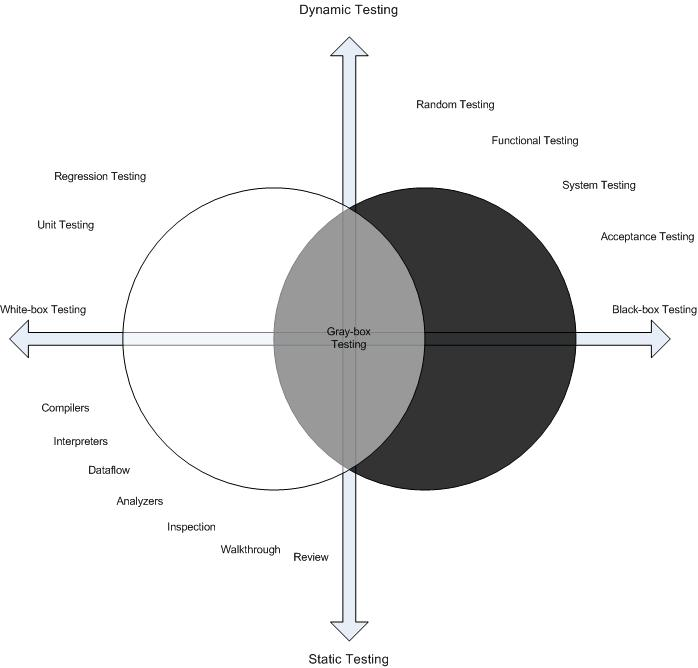
\includegraphics[width=16cm, height=12cm ]{Literature/Drawing34.jpg}
%	\caption{Software Testing Workflow}
%\end{center}  
%\end{figure}


%We have explained software testing graphically with the help of plotting venn diagram on two dimensional axis. The positive x axis represent black-box while negative x axis represent white-box testing. Grey-box testing in the middle is represented by the overlapping of black-box and white-box testing. Similarly on positive y axis we have dynamic testing and on negative y axis we have static testing.
%Now if a test is black box and dynamic then the test will fall in 0 to 90 degree on the diagram and if the test is black-box and static then it will fall in 270 to 360 degree. On the other hand if the test is white-box and dynamic then it will fall in 90 to 180 degree and if the test is white-box and static then it will fall in 180 to 270 degrees.




\subsection{Software Testing Execution}
Testing process can be divided into static and dynamic phases on the basis of test execution. In static testing test cases are analysed statically for checking errors without test execution. In addition to software code, high quality softwares are accompanied by necessary documentation. It includes requirements, design, technical, user manual marketing information. Reviews, walkthroughs or inspections are most commonly used techniques for static testing. In dynamic testing the software code is executed and input is converted into output. Results are analysed against expected outputs to find any error in the software. Unit testing, integration testing, system testing, and acceptance testing are most commonly used as dynamic testing methods~\cite{fairley1978tutorial}.

%Dynamic testing can be manual or automated. In manual testing the programmer develops the test cases which are executed by the developed software to find any error in processing or output. Similarly in automated testing the software or components of the software is given as input to testing software that automatically generates test cases and executes the SUT against them to find any errors. Manual testing typically consumes more time and resources than automated testing.



\subsection{Manual Testing}
Manual testing is the technique of finding faults in software in which the tester writes the code by hand to create test cases and test oracle~\cite{Ciupa2008}. Manual testing may be effective in some cases but it is generally laborious, time consuming and error-prone~\cite{tretmans1999}. Additionally, it requires that the testers must have appropriate skills, experience and sufficient knowledge of the SUT for evaluation from different perspectives.
 
\subsection{Automated Testing}
Automated testing is the technique of finding faults in a software in which the test cases or test oracle are generated automatically by a testing tool~\cite{Leitner2007}. There are tools which can automate part of a test process like generation of test cases or execution of test cases or evaluation of results while other tools are available which can automate the whole testing process. The use of automated testing made it possible to test large volumes of code, which would have been impossible otherwise~\cite{ramamoorthy1975}.

%\section{Automated Random Testing}
%\subsection{Test Data Generation}
%\subsection{Test Execution}
\subsection{Test Oracle}
Test oracles set the acceptable behaviour for test executions~\cite{baresi2001test}. All software-testing techniques depend on the availability of test oracle~\cite{gaudel2010software}. Designing test oracle for ordinary software may be simple straightforward. However, for relatively complex software designing of oracle is quite cumbersome and requires special ways to overcome the oracle problem. Some of the common issues in the oracle problem include:
\begin{enumerate}
\item The assumption that the test results are observable and can be compared with the oracle.
\item An ideal test oracle would satisfy desirable properties of program specifications~\cite{baresi2001test}.
\item A specific oracle to satisfy all conditions is seldom available as rightly pointed out by Weyuker who ?states that truly general test oracles are often unobtainable Weyuker~\cite{weyuker1982testing} 
\end{enumerate}
%\subsection{Test Report}



\section{Random Testing}
Random testing is a dynamic black-box testing technique in which the software is tested with non-correlating or unpredictable test data from the specified input domain~\cite{Chan2002}. The input domain is a set of all possible inputs to the software under test. According to Richard~\cite{hamlet1994}, in random testing, input domain is first identified, then test points are randomly taken from the whole input domain by means of random number generator. The program under test is executed on these points and the results obtained are compared with the program specifications. The test fails if the results are not according to the specifications and vice versa. Failure of any test results reflects error in the SUT.
\begin{figure}[h]
	\centering
	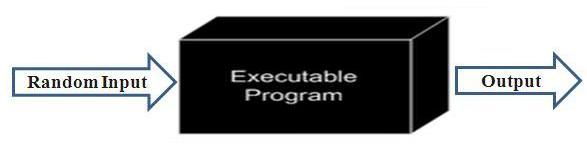
\includegraphics[scale=0.5]{Literature/randomTesting.jpg}
	\caption{Random Testing}
\end{figure}

Generating test data by random generator is quite economical and requires less intellectual and computational efforts~\cite{Ciupa2008a}. This feature makes it an ideal choice for use in automated testing tools [---]. Moreover, the no human intervention is involved in data generation that ensures an unbiased testing process.

However, generating test cases with out using any background information makes random testing susceptible to criticism. It is criticized for generating many test cases ending up at the same state of software. It is further stated that, random testing generates test inputs that violates requirements of the given SUT making it less effective~\cite{sen2007effective},~\cite{pacheco2009directed}. Myers mentioned random testing as one of the least effective testing technique~\cite{Myers1979}.

It is stated by -------- that Myers statement was not based on any experimental evidence. Later experiments performed by several researchers~\cite{hamlet1994},~\cite{Ciupa2008},~\cite{leitner2007efficient} and~\cite{Duran1981} confirmed that random testing is as effective as any other testing technique. It was found experimentally~\cite{Duran1981} that random testing can also discover subtle faults in a given SUT when subjected to large number of test cases. It was pointed out that the simplicity and cost effectiveness of random testing makes it more feasible to run large number of test cases as opposed to systematic testing techniques which require considerable time and resources for test case generation and execution. The empirical comparison proves that random testing and partition testing are equally effective~\cite{hamlet1990} A comparative study conducted by Ntafos~\cite{ntafos1998random}. concluded that random testing is more effective as compared to proportional partition testing.


\section{Various versions of random testing}
Researchers have tried various approaches to bring about improvement in the performance of random testing. The prominent modifications in random strategy are stated below:

\subsection{Adaptive Random Testing}
Adaptive random testing (ART), proposed by Chen et al.~\cite{Chen2008} is based on the previous work of Chan et al.~\cite{Chan1996}regarding the existence of failure patterns across the input domain. Chan et al observed that failure inducing inputs in the whole input domain form certain geometrical patterns and divided these into point, block and strip patterns described below.

\begin{enumerate}
\item Point pattern: In the point pattern inputs inducing failures are scattered across the input domain in the form of stand-alone points. Example of point pattern is the division by zero in a statement total = num1/num2; where num1, num2 and total are variables of type integer.
\item Block pattern: In the block pattern inputs inducing failures lie in close vicinity to form a block in the input domain. Example of block pattern is failure caused by the statement if ( (num \textgreater 10) \&\& (num \textless 20) ). Here 11 to 19 are a block of faults.
\item Strip pattern: In the strip pattern inputs inducing failures form a strip across the input domain. Example of strip pattern is failure caused by a statement num1 + num2 = 20. Here multiple values of num1 and num2 can lead to the fault value 20. 
\end{enumerate}

\begin{figure}[h]
	\centering
	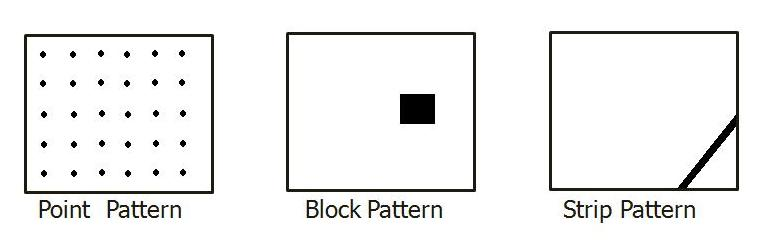
\includegraphics[scale=0.5]{Literature/pointblockstrip.jpg}
	\caption{Patterns of failure causing inputs}
	\label{fig:patterns2}
\end{figure}

In figure~\ref{fig:patterns2} the square boxes indicate the whole input domains. The white space in each box shows legitimate and faultless values while the black colour in the form of points, block and strip inside the respective box each box indicates the point, block and strip fault patterns.

Chen et al. ~\cite{Chen2008} argued that ordinary random testing might generate test inputs lurking too close or too far from the input inducing failure and thus fails to discover the fault. To generate more faults targeted test inputs they proposed Adaptive Random Testing (ART) as a modified version of ordinary random testing where test values are selected at random as usual but are evenly spread across the input domain by using two sets. The executed set comprises the test cases executed by the system and the candidate set includes the test cases to be executed by the system. Initially both the sets are empty. The first test case is selected at random from the candidate set and stored in executed set after execution. The second test case is then selected from the candidate set which is far away from the last executed test case. In this way the whole input domain is tested with greater chances of generating test input from the existing fault patterns.

In the experiments conducted by Chen et al.~\cite{Chen2008} the number of test cases required to detect first fault (F-measure) was used as a performance matrix instead of the traditional matrix P-measure and E-measure. Experimental results using ART showed up to 50\% increase in performance compared to ordinary random testing. The authors admitted that the issues of increase overhead, spreading test cases across the input domain for complex objects and efficient ways of selecting candidate test cases still exist. Chen et al continued their work on ART to address some of these issues and proposed its upgraded version in~\cite{chen2009enhanced} and~\cite{Chen2005}. 

\subsection{Mirror Adaptive Random Testing}
%As discussed in the above section ART provide better results, however the increase in overhead due to extra computation to achieve even spread of test inputs makes it less cost effective. 
Mirror Adaptive Random Testing (MART)~\cite{Chen2003} is an improvement on ART by using mirror-partitioning technique to decrease the extra computation involved in ART and reduce the overhead.

\begin{figure}[h]
\begin{center}
	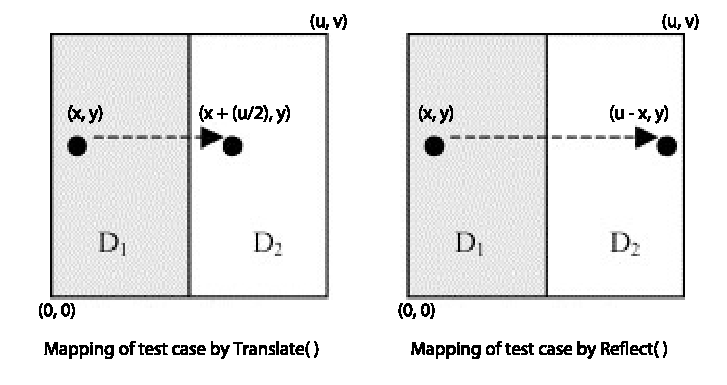
\includegraphics[width=13cm, height=6cm ]{Literature/mart2.pdf}
	\caption{Mirror Adaptive Random Testing~\cite{Chen2003}}
\label{fig:mirrorART}
\end{center}  
\end{figure}

In this technique, the input domain of the program under test is divided into n disjoint sub-domains of equal size and shape. One of the sub-domains is called source sub-domain while all the others are termed as mirror sub-domains. ART is then applied only to the source sub-domain to select the test cases while from all other sub-domains test cases are selected by using mirror function. In MART {(0, 0), (u, v)} are used to represent the whole input domain where (0, 0) is the leftmost and (u, v) is the rightmost top corner of the two dimensional rectangle. On splitting it into two sub-domains we get {(0, 0), (u/2, v)} as source sub-domain and {(u/2, 0), (u, v)} as mirror sub-domain. Let suppose we get x and y test cases by applying ART to source sub-domain, now we can linearly translate these test cases to achieve the mirrored effect, i.e. (x + (u/2), y) as shown in the figure~\ref{fig:mirrorART}. Comparative study of MART with ART provide evidence of equally good results of the two strategies with MART having the added advantage of using only one quarter of the calculation as compared with ART and thereby reduces the overhead.


\subsection{Restricted Random Testing}
Restricted Random Testing~\cite{chan2003normalized} is another approach to overcome the problem of extra overhead in ART. Restricted Random Testing (RRT) achieves this by creating a circular exclusion zone around the executed test case. A candidate is randomly selected from the input domain for the next test case. Before execution the candidate is checked and discarded if it lies inside the exclusion zone. This process repeats until a candidate laying outside the exclusion zone is selected. This ensures that the test case to be executed is well apart from the last executed test case. The radius of exclusion zone is constant around each test case and the area of each zone decreases with successive cases.

\begin{figure}[h]
	\centering
	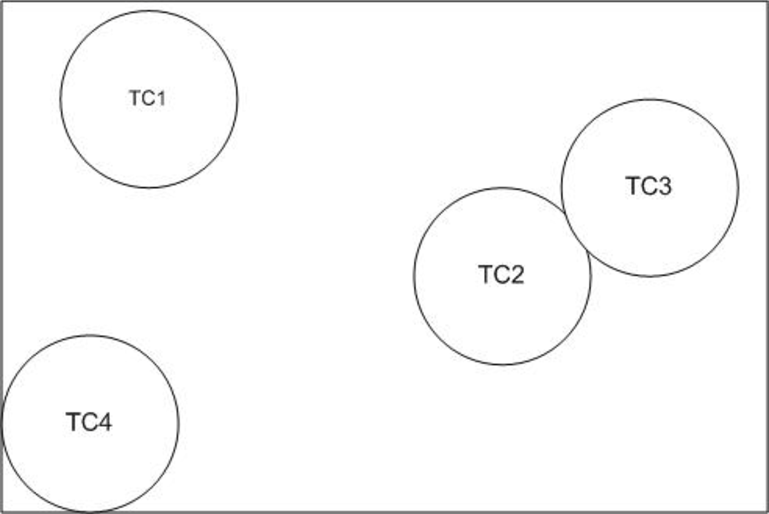
\includegraphics[width= 6cm, height = 5cm]{Literature/RRT.pdf}
	\caption{Input domain with exclusion zone around the selected test case}
\end{figure}

To find the effectiveness of RRT, the authors compared it with ART and RT on 7 out of the 12 programs evaluated by ART and MART. The experimental results showed that the performance of RRT increases with the increase in the size of the exclusion zone and reaches the maximum level when the exclusion zone is raised to largest possible size. %Normalized Restricted Random Testing~\cite{chan2003normalized} is an improvement over RRT by allowing the testers to have better information about the target exclusion rate (R) of RRT. 
They further found that RRT is up to 55\% more effective than ordinary random testing in terms of F-measure (Where F-measure is the total number of test cases required to find the first failure).



\subsection{Directed Automated Random Testing}
Godefroid et al.,~\cite{Godefroid2005} proposed Directed Automated Random Testing (DART). %Its main purpose was to overcome the cost and difficulty of manual testing while keeping its quality intact. It automate the whole testing process including generation of unit tests, test drivers/harness and assertions for functional correctness. 
The main features of DART can be divided into the following three parts:
\begin{enumerate}
\item Automated Interface Extraction: DART automatically identifies external interfaces of a given SUT. These interfaces include external variables, external functions and the user-specified main function, which initializes the program execution.
\item Automatic Test Driver: DART generate test drivers to run the test cases. All the test cases are randomly generated according to the underlying environment.
\item Dynamic Analysis of execution: The DART instruments the given SUT at the start of the process in order to track its behaviour dynamically at run time. The results obtained are analysed in real time to systematically direct the test case execution along alternative path for maximum code coverage.
\end{enumerate}

The DART algorithm is implemented in the tool which is completely automatic and accepts the test program as input. After the external interfaces are extracted it then use the pre-conditions and post-conditions of the program under test to validate the test inputs. For languages that do not support contracts inside the code (like C), they used public methods or interfaces to mimic the scenario —————————- to be continued

\subsection{Quasi Random Testing}
Quasi-random testing (QRT)~\cite{Chen2005} is a testing technique which takes advantage of failure region contiguity by distributing test cases evenly with decreased computation. %Chan et al after the analysis of faults in various experiments found that the fault patterns across the input domain are continuous. 
To achieve even spreading of test cases, QRT uses a class with a formula, that forms an s-dimensional cube in s-dimensional input domain and generates a set of numbers with small discrepancy and low dispersion. The set of numbers is then used to generate random test cases that are permuted to make them less clustered and more evenly distributed. An empirical study was conducted to compare the effectiveness of QRT with ART and RT. The empirical results of the experiments showed that in 9 out of 12 programs QRT found a fault quicker than ART and RT while there was no significant improvement in the remaining three programs.
%\subsection{Monti Carlo Random Testing}

%\subsection{Good Random Testing}

\subsection{Feedback-directed Random Testing}
Feedback-directed Random Testing (FDRT)~\cite{Pacheco2007} is a technique that generate unit test suite at random for object-oriented programs. As the name implies FDRT uses the feedback received from the execution of first batch of randomly selected unit test suite to generate next batch of more directed unit test suite. In this way redundant and illegal unit tests are eliminated incrementally from the test suite with the help of filtration and application of contracts. For example unit test that produce IllegalArgumentException on execution is discarded, because, selected argument used in this test was not according to the type of argument the method required. 

\subsubsection{Randoop: Feedback-directed Random Testing}
The FDRT technique is implemented in Random tester for Object Oriented Programs (RANDOOP) tool~\cite{Pacheco2007b}. RANDOOP is a fully automatic tool, capable of testing Java classes and .Net binaries which takes a set of classes (java or .Net executable), contracts, filters and time limit as input and gives output as a suite of JUnit and NUnit for Java and .Net programs respectively. Each unit test in a test suite is a sequence of method calls (hereafter referred as sequence). RANDOOP build the sequence incrementally by randomly selecting a public method from the class under test and arguments for these methods are selected from the predefined pool in case of primitive types and a sequence or null value in case of reference type. RANDOOP maintains two sets called ErrorSeqs and NonErrorSeqs to record the feedback. It extends ErrorSeqs set in case of contract or filter violation and NonErrorSeqs set when no violation is recorded in the feedback. The use of this dynamic feedback evaluation at runtime brings an object to very complex and interesting state. On test completion it produce ErrorSeqs and NonErrorSeqs as JUnit/NUnit test suite. In terms of coverage and number of faults discovered, RANDOOP implementing FDRT was compared with random testing of JCrasher and JavaPathFinder~\cite{visser2004test}. In the experiments 14 libraries of both Java and .Net were evaluated. The results showed that RANDOOP achieved more coverage than JCrasher in behavioural, branch coverage and faults detection. It can achieve on par coverage with systematic approaches like JavaPathFinder. RANDOOP also has an edge over model checking for its ability to easily search large input domains.
%\subsection{Adaptive Random Testing for Object-Oriented}



\subsection{Object Distance and its application}
To improve the performance of random testing the emphasis of ART was on the distance be- tween the test cases. But this distance was defined only for primitive data types like integers and other elementary input. Ciupa et al defined the parameters that can be used to calculate distance between the composite programmer-defined types so that ART can be applicable to testing of today’s object-oriented programs~\cite{Ciupa2006}. Two objects have more distance between them if they have more dissimilar properties. The parameters to specify the distance between the objects are dynamic types, values of its primitive and reference fields. Strings are treated as a directly usable values and Levenshtein distance~\cite{Levenshtein1966} that is also known as edit distance is used as a distance criteria between the two strings. To implement object distance first all the distances of the objects are measured. Then two sets candidate- objects containing the all the objects ready to be run by the system and the used-objects set, which is initially empty. First object is selected randomly from the candidate-object set and is moved to used-object set when executed by the system. Now the second object selected from the candidate set for execution is the one with the biggest distance from the last executed object present in the used-object set. This process is continuing until the bug is found or the objects in the candidate-object set are finished.

\subsubsection{ARTOO Tool}
After the criteria to calculate the distance between the objects is defined~\cite{Ciupa2006}, the same team implemented that model and performed several experiments to evaluate the proposed model. Adaptive Random Testing for Object Oriented (ARTOO) is a testing strategy, based on object distance, implemented in AutoTest tool \cite{16 search it Mendeley}.
ARTOO was implemented as a plug-in strategy in AutoTest. It only deals with creating and selecting inputs and all other functionality of the AutoTest was the same. Since ARTOO is based on object distance therefore the method for test input selection is to pick that object from the candidate set (A pool of objects that is a potential candidate to be executed by the system) that has the highest average distance in comparison to the objects already executed. In the experiments classes from EiffelBase library \cite{17 search it mendeley} were used. To evaluate ARTOO the same tests were also applied to directed random strategy (RAND). The outcome of the experiments showed that ARTOO finds the first bug with fewer test cases than RAND. The computation to select test case in ARTOO is more than RAND and therefore ARTOO takes more time to generate a test input. The experiments also found few of the bug found by ARTOO were not pointed out by RAND furthermore ARTOO is less sensitive to the variation of seed value than RAND.

\subsubsection{Experimental Assessment of RT for Object-Oriented Software}
In this research the effect of various parameters involved in random testing and its effect on efficiency is evaluated by performing various experiments on Industrial-grade code base. Large-scale clusters of computers were used for 1500 hours of CPU time which resulted in 1875 test sessions for 8 classes under test.~\cite{Ciupa2007} The finding of the experiments are 1. Version of random testing algorithm that is efficient for smaller testing timeout is equally efficient for higher testing timeouts. 2. The value of seed for random testing algorithm plays a vital role in finding the number of bugs in specific time. 3. Most of the bugs are found in the first few minutes of the testing sessions.


%\section{Automated Random Testing Tools}
\section{Tools for Automated Random Testing}
From the literature we can find a number of open source and commercial testing tools that automatically generate unit tests. Each tool utilize different generation technique but the one we are interested in is random technique. We present the most well known tools.


\subsection{JCrasher}

JCrasher is first of the three automatic testing tools developed by Csallner C. and Smaragadakis Y.~\cite{Pacheco2007b}. As the name suggests JCrasher tries to crash the Java program with random input and any exceptions thrown during the process are recorded. All exceptions are then compared to the list of acceptable exception, which are defined in advance as heuristics; any undefined/un- declared runtime exceptions are considered errors. Since programs interact with the world through its public methods and they are also exposed to different kind of inputs, therefore, JCrasher tests only these methods with random inputs.

\begin{figure}[h]
	\centering
	\includegraphics[width=15cm, height=7cm]{Literature/JCrasher.png}
	\caption{Process of robustness testing of Java program with JCrasher~\cite{Pacheco2007b}}
	\label{fig:JCrasher}
\end{figure}

Figure~\ref{fig:JCrasher} illustrate the working of JCrasher by testing a java program namely T.java. The source file is first compiled using javac and the obtained byte code is passed into JCrasher. The JCrasher using Java reflection~\cite{chan1999java}  analyse all the methods declared by class T and by their transitive parameter types P to generate the most appropriate test data set. The test data set is written to a file TTest.java that is compiled and executed by JUnit. All the exceptions produced during test case executions are collected and compared with robustness heuristic to check for violation. Any violated test case is reported as error.\\

JCrasher is a pioneer to perform fully automatic testing from test case generation, execution, filtration to reporting the results. One of its novelty  is that it generates test case as JUnit files that can be easily read and can be used for regression testing. Another important feature of JCrasher is to execute each new test on a ``clean slate" ensuring that the changes made by the previous tests do not affect the new test.  

% check parameter space or parameter graph in the figure???


\subsection{Jartege}
Jartege (\uline{Ja}wa \uline{r}andom \uline{te}st \uline{ge}nerator)~\cite{Oriat2004} is an automated testing tool that randomly generates unit tests for Java classes with contracts specified in Java Modelling Language (JML). The contracts include methods pre- and post-conditions and class invariants. Initially Jartege uses the contracts to eliminate irrelevant test cases and later on the same contracts serve as test oracle to differentiate between errors and false positives. Jartege uses simple random testing to test classes and generate test cases, however, it facilitate to parametrise its random aspect in order to prioritise testing specific part of the class or to get interesting sequences of calls. These includes: 
\begin{itemize}
\item To define the operational profile of the classes i.e. the likely use of the class under test by other classes.  
\item To define the weight of each class and method under test and give test priority to the one's with highest weight and skip those with null weight.
\item To control the creation of newly created objects with creation probability functions. Low probability means creation of fewer objects and more re-usability for different operations while high probability means numerous new objects with less re-usability.
\end{itemize}

\noindent The Jartege technique evaluate class by entry pre-condition and internal pre-condition. Entry pre-conditions are the contracts which must be met by the generated test data to test the method while internal pre-conditions are the ones which are inside the methods and their violation are considered error either in method or in the specification. The benefits of Jartege is that it checks for errors in both program and specifications and the Junit tests produced by Jartege can be used later as regression tests. Its minor short coming is that the SUT JML specifications must exist or may be written manually in order to be tested by Jartege.

\subsection{Eclat}
Eclat~\cite{Pacheco2005} testing tool automatically generates and classify unit tests for Java classes. The process can be divided into three main components. In the first component, it selects small subset of test inputs, likely to reveal faults in the given SUT, from a large set of test inputs.

\begin{figure}[h]
	\centering
	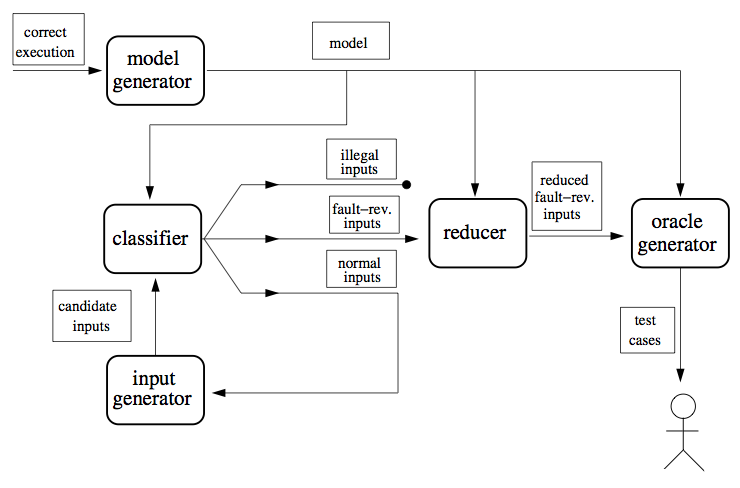
\includegraphics[width=15cm, height=9cm]{Literature/eclat_working.png}
	\caption{Main component of Eclat contributing to generate test input~\cite{Pacheco2005}}
	\label{fig:eclat}
\end{figure}


\noindent The tool takes a software and a set of test cases for which the software runs properly. It then creates an operational model based on the correct software operations and apply the test data to it. As a result any inputs whose operational pattern of execution differs from the operational model are (1) likely to reveal fault in the given SUT, (2) Likely to produce normal operations despite violating the model, (3) illegal input that the program is not required to handle. In the second component, reducer function is used to discard any redundant input, leaving only one input per operational pattern.The third and final component facilitate automated testing by converting the acquired test inputs into test cases and creation of oracle to determine whether the test succeeds or fail. \\
\indent To measure the effectiveness, the researchers tested 9 programs on both Eclat and JCrasher~\cite{Pacheco2007b}.  The experimental results revealed that Eclat outperformed JCrasher. On average, Eclat selected 5.0 inputs per run, and 30\% of those revealed a fault. While JCrasher selected 1.13 inputs per run, and 0.92\% of those revealed a fault. The short coming of Eclat is its dependence on the initial pool of correct test cases which is usually written manually and existence of any errors in it can propagate and affect the whole testing process.    

%\subsection{JTest}
%Parasoft Jtest is a commercial tool that automatically generates and execute unit tests. It can be easily integrated to Java IDEs like Eclipse where it provide two main functionalities, i.e. Static Analysis, Unit testing and code coverage. [25]
%In static analysis Jtest takes a complete project or set of classes as input and compares it with a list of built-in rules. The statement violating any of these rules is an error. It also suggests probable fixes for the detected fault.
%For unit testing it takes a class as an input and processes a number of scenarios against it to generate and execute unit tests. Once unit tests are executed they become the part of regression test for future reference.
%Jtest also shows the code coverage of the program by colour coding the statements that are not executed by the unit tests.

\subsection{QuickCheck}
QuickCheck~\cite{Claessen2000} is a lightweight random testing tool that can be used for testing of Haskell programs~\cite{Hudak2007}. Haskell is a functional programming language where programs are evaluated using expressions rather than statements as in the case of imperative programming. Since in Haskell most of the functions are pure other than IO functions, therefore it focuses on testing pure functions. These are the functions which depends upon its input parameters and make changes to them only. \\
QuickCheck takes as input the testers defined properties of the program called Haskell functions and the program to be tested. The tool uses built-in random generator to generate test data or the tester may provide custom define test data generator. Any generated test inputs that satisfies Haskell functions are declared as valid tests input. To cope with oracle problem, the authors have designed a simple domain-specific language of testable specifications embedded in Haskell. The tester use it to define expected properties of the functions under test. QuickCheck then checks and declare a fault in the function where a test case violate these properties.   


%\subsection{AgitarOne}
%AgitarOne is a commercial tool that automatically generates unit tests. It has a Junit Generator engine that can create 25,000 lines or more of Junit per hour [29]. It can be easily integrated into famous IDE like Eclipse. It takes as input, classes under test, time and optionally any knowledge or test cases that has a positive influence on the performance of the testing process. The generated Junit tests can be run from the same IDE and can also be used for later regression testing. The GUI interface is called a dashboard which provides in depth knowledge of the tests conducted, failures detected, alerts and the archieves of the tests conducted earlier. It also shows the coverage obtained after executing the Junits against the code under test.

\subsection{Autotost}
Based on Formal Automated testing AutoTest is a tool used for testing of Eiffel programs~\cite{Ciupa2007}. The Eiffel language use the concept of contracts (pre-conditions, postconditions and class invariants). Input can be a single class, method or a set of classes which is then processed by AutoTest to generate test cases. It generates both primitive and object type test cases. All the generated test cases are kept in a pool and then randomly a test case is selected from it for execution. A user can set the features of the AutoTest options include: Number of test cases to generate, whether to monitor pre or post condition, order of testing and the initial values of the primitives variables.

\subsection{TestEra}
TestEra~\cite{Khurshid2004} is a novel framework for testing Java applications. All the tests are produced and executed in an automated fashion. Tests are conducted on the basis of the method specifications~\cite{Chang1999}. TestEra takes methods specifications, integer value as a limit to the generated test cases and the method under test. It uses pre-conditions of a method from specifications to automatically generate test cases up to the specified limit. These test cases are then executed on the method and the result is compared against the postconditions (oracle) of that method. Any test case that fails to satisfy postcondition is considered as a fault. The complete error log is displayed in the Graphical User Inteface (GUI).

\subsection{Korat} % please read thesis of khurshid in Mendeley in phd thesis section for more information.
Korat~\cite{Boyapati2002} is a novel framework for automated testing of Java programs based on their formal specifications~\cite{chang1999structural}. As the test start, it uses methods pre-condition to generate all non-isomorphic test cases up to a given size. It then executes each of the test case and compare the obtained results to the methods post-condition, which serves as an oracle to evaluate the correctness of each test case. Korat uses a black-box testing approach where it uses methods pre-conditions as predicates. After the Java predicates and finitization (that bounds the predicates input space) are defined, Korat systematically explore the predicates input space and generate all non isomorphic inputs for which the predicates return true. The core part of Korat monitors execution of the predicates on candidate inputs to filter the inputs based on the fields accessed during executions.  
  



\section{YETI}
York Extensible Testing Infrastructure (YETI) is an automated tool for testing Java, JML and .NET assemblies~\cite{Oriol2010c}. YETI execute the program under test with random generated but type-correct inputs and declare a fault if the response is an unexpected exception or a contract violation. YETI has been designed with an emphasis on extensibility. Its three main parts: the core infrastructure, strategies and language bindings are loosely coupled to easily accommodate new languages and strategies. To keep the process fully automated YETI uses two approaches for oracle (pass/fail judgement). If available, YETI uses code contracts as oracle if not it uses undeclared runtime exceptions of the underlying language as oracle. The test cases revealing errors are reproduced at the end of each test session for unit and regression testing. Other prominent features of YETI include its Graphical User Interface (GUI) for user friendliness and ability to distribute large testing tasks in cloud for parallel execution~\cite{Oriol2010}. The following sections briefly describe internal working and execution of YETI tool. 

\subsection{Construction of Test Cases}
YETI construct test cases at random by creating objects of the class under test and randomly calling its methods with inputs according to its parameter's-space. Strategy section contains seven different strategies and inputs to the tested methods is defined by one of the selected strategy. To completely automate the data generation YETI   split input values into two types i.e. primitive data types and user defined classes. For Java primitive data types, which includes short, byte, char, int, float, double, long etc., YETI uses its own built-in random value generation library. However, in the case of user defined classes where objects data type is a user defined class YETI calls its constructor to generate object of that class at run time. It may be possible that the constructor require another object and in this case YETI will recursively calls the constructor of that object. This process is continued until the an object with blank constructor, constructor with only primitive types (type 1) or the set level of recursion is reached. 

\subsection{Command-line Options}
While YETI GUI launcher has been developed during this research study, to take maximum benefit of the available options one still need to launch YETI from CLI mode. These command-line options are case insensitive and can be provided as input to the tool in CLI mode. For example, to save processing power command line option -nologs can be used to bypass real-time logging. The following table describes few of the most common command-line options available in YETI.    

\begin{table}[h]
%\scriptsize
\caption{YETI command line options} % title of Table
\smallskip
\centering % used for centering table
\begin{tabular}{ll } % centered columns (4 columns)
\hline

Levels 					&Purpose 			\\
\hline
-java						&Test programs coded in Java	 	\\
-jml						&Test programs coded in JML			\\
-dotnet					&Test programs coded in .NET		\\
-ea						&To check code assertions \\
-nTests					&Specify number of tests after which the test stops	\\
-time						&Specify time in seconds or minutes after which the test stops\\
-testModules				&Specify one or more modules to test 	\\
-rawlogs					&Prints real time logs during test \\
-nologs					&Omit real time logs and print end result only\\
-yetiPath					&Specify path to the test modules\\ 
-gui						&Show test session in GUI\\
-DSSR					&Specify Dirt Spot Sweeping Random strategy for this session\\
-ADFD					&Specify Automated Discovery of Failure Domain strategy for this session\\
-random					&Specify random test strategy for this session\\
-randomPlus				&Specify random plus test strategy for this session\\
-randomPlusPeriodic		&Specify random plus periodic test strategy for this session\\
-nullProbability				&Specify probability of inserting null as input value\\
-newInstanceProability		&Specify probability of inserting new object as input value\\

\hline %inserts single line
\end{tabular}
\bigskip
\label{table:cliOptions} % is used to refer this table in the text
\end{table}


\subsection{YETI Execution}
YETI being developed in Java is highly portable and can easily run on any operating system with Java Virtual Machine (JVM). YETI can be executed from both command line and GUI. To build and execute YETI, it is necessary to specify the project and all the .jar library files particularly javassist.jar in the CLASSPATH or JVM would not be able to find and execute it. There are several options available as discussed in section xxx??? to accommodate specific needs but the typical command to invoke YETI is given in figure~\ref{fig:XXX???}. In this particular command YETI tests java.lang.String and yeti.test.YetiTest modules, for details of other options please see section xxx????. 

\begin{figure}[h]
	\centering
	\frame{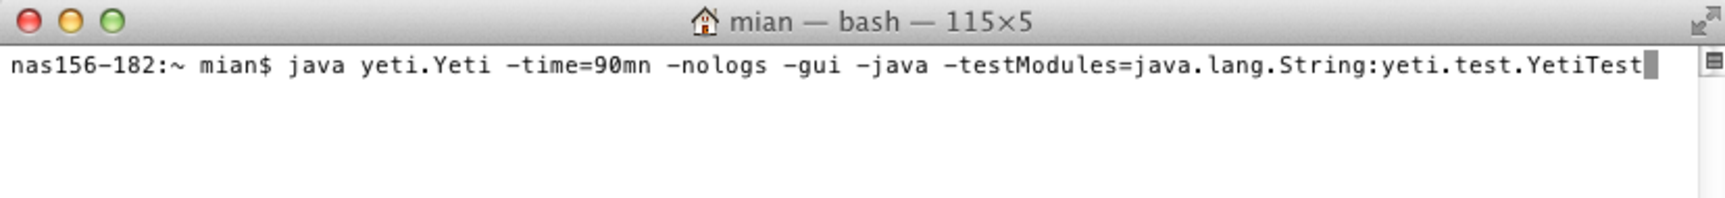
\includegraphics[width= 14cm, height = 1.8cm]{Literature/yetiCommandCLI.pdf}}
	\caption{Command to launch YETI from CLI}
\end{figure}

Alternately, runnable jar file by the name YetiLauncher is also available to launch YETI from GUI. However, till the writing of this thesis, the GUI version of YETI only supports the basic options of YETI. Figure xxx??? shows the equivalent of above command in GUI mode.

\begin{figure}[h]
	\centering
	\frame{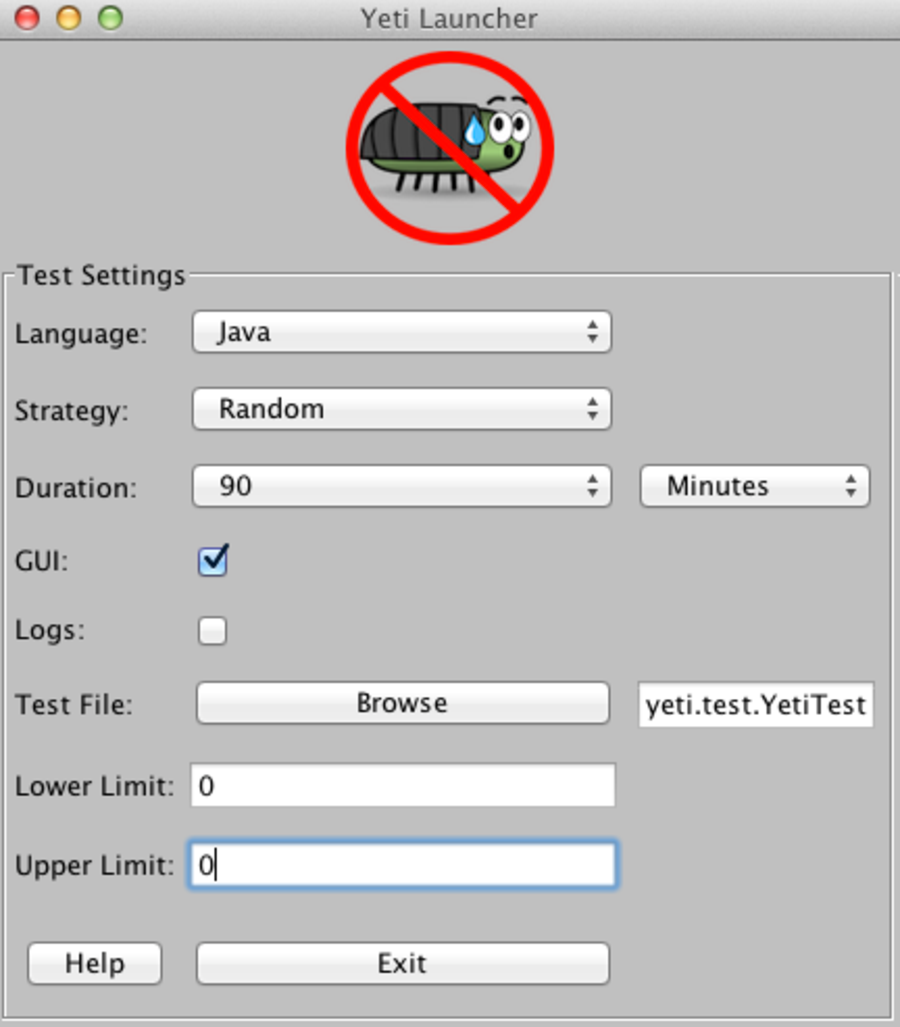
\includegraphics[width= 7cm, height = 8cm]{Literature/yetiCommandGUI.pdf}}
	\caption{Command to launch YETI from GUI}
\end{figure}


As a result of both the above commands YETI launch its own GUI window and start testing the assigned programs. 




\subsection{YETI Report}



\subsection{Summary of automated testing tools}


\begin{figure}[h]
	\centering
	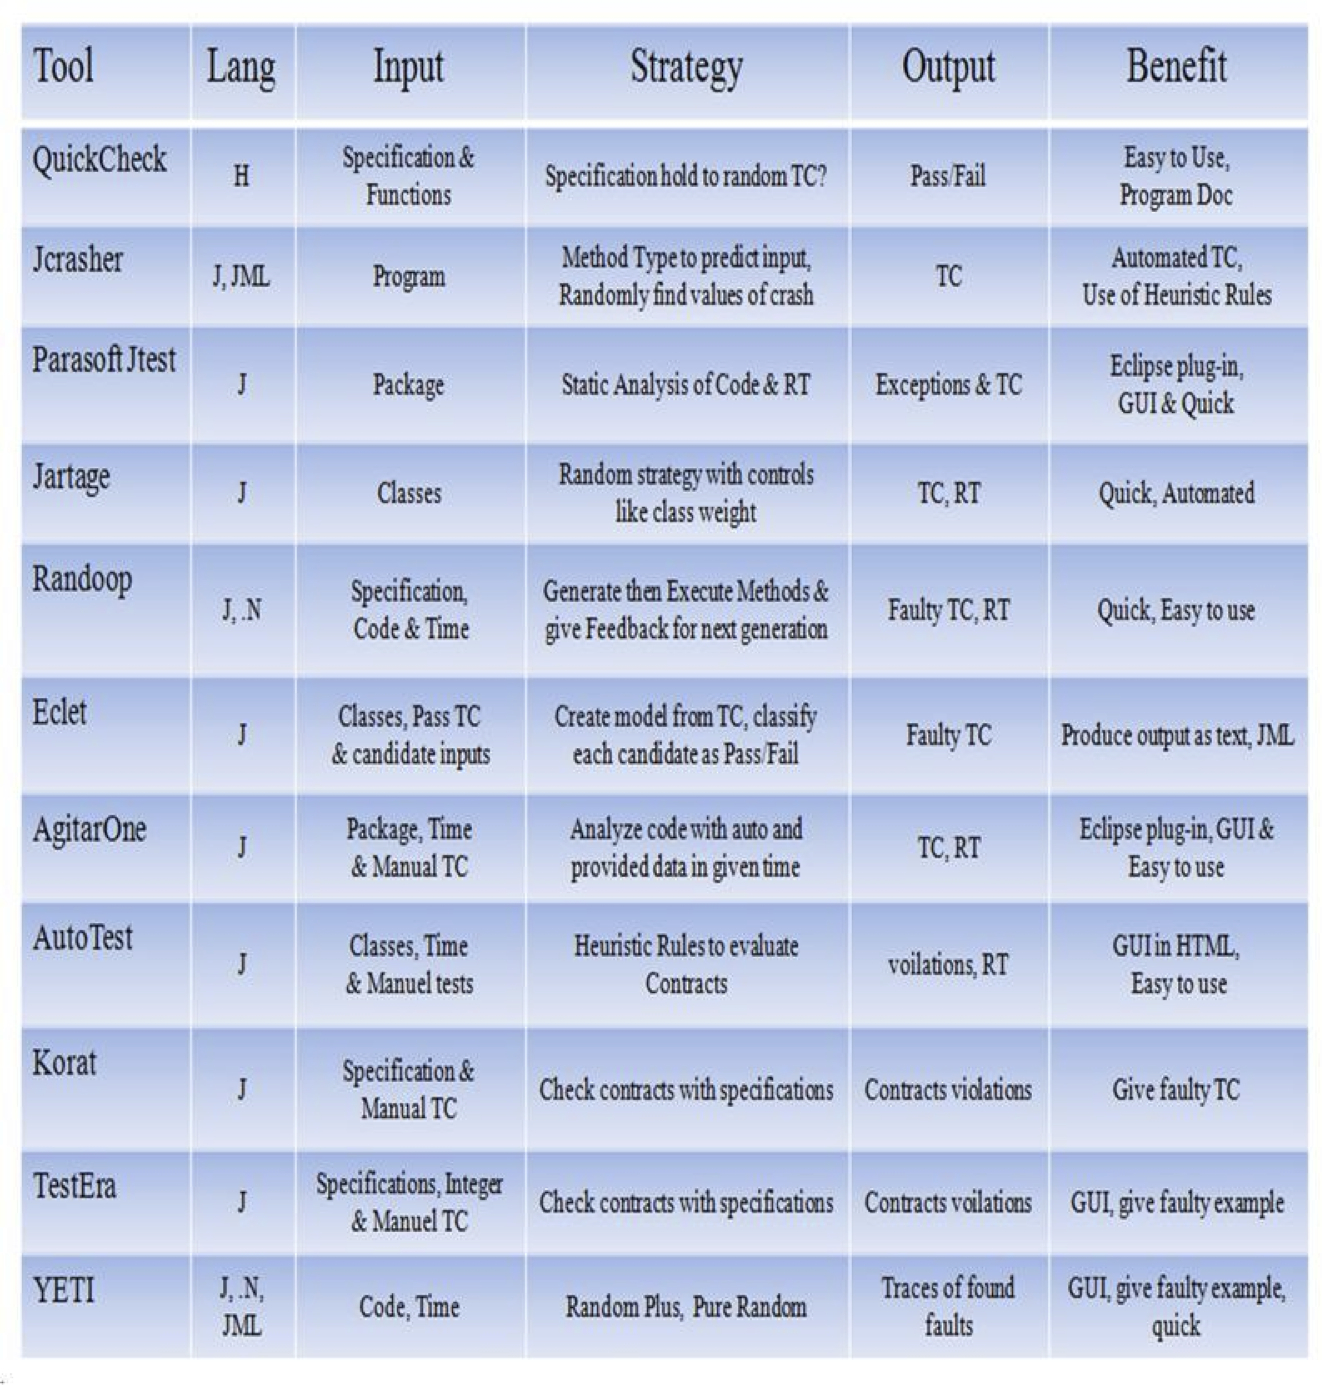
\includegraphics[scale=0.6]{Literature/tools.jpg}
	\caption{Summary of automated testing tools}
\end{figure}


\section{Conclusion}


% ------------------------------------------------------------------------


%%% Local Variables:
%%% mode: latex
%%% TeX-master: "../thesis"
%%% End:
